% NeurIPS 2026 poster for Mixture-of-Control.
% Main-conference format: 140 cm x 90 cm, landscape.

\documentclass[final]{beamer}

% ====================
% Packages
% ====================

\usepackage[T1]{fontenc}
\usepackage{lmodern}
\usepackage[size=custom,width=140,height=90,scale=1.0]{beamerposter}
\usetheme{gemini}
\usecolortheme{neurips}
\usepackage{graphicx}
\usepackage{booktabs}
\usepackage{tabularx}
\usepackage{array}
\usepackage{tikz}
\usetikzlibrary{positioning}
\usepackage{qrcode}
\usepackage{anyfontsize}

% ====================
% Paper metadata
% ====================

\newcommand{\papertitle}{Mixture-of-Control: State-Aware Fine-Tuning for Transformer-based Models}
\newcommand{\paperid}{NeurIPS 2026 \#148178}
\newcommand{\paperurl}{https://neurips.cc/virtual/2026/loc/sydney/poster/148178}
\newcommand{\arxivurl}{https://arxiv.org/abs/2606.31397}

\title{\papertitle}
\author[Nguyen, Luu, Pham, Tran]{\texorpdfstring{%
  Duc-Anh Nguyen\inst{1,2}\textsuperscript{*,\dagger}
  \and Tien Ngoc Luu\inst{1}\textsuperscript{*}
  \and Tung Pham\inst{1}
  \and Toan Tran\inst{1}%
}{Duc-Anh Nguyen, Tien Ngoc Luu, Tung Pham, Toan Tran}}
\institute[Qualcomm AI Research; University of Virginia]{%
  \inst{1} Qualcomm AI Research
  \samelineand \inst{2} University of Virginia
  \\[-0.1ex]\footnotesize
  * Equal contribution \quad
  \dagger Work done during an internship at Qualcomm \quad
  Corresponding author: Toan Tran}

% ====================
% Layout
% ====================

% Four separators and three columns fill the paper width.
\newlength{\sepwidth}
\newlength{\colwidth}
\setlength{\sepwidth}{0.021\paperwidth}
\setlength{\colwidth}{0.30533\paperwidth}
\newcommand{\separatorcolumn}{\begin{column}{\sepwidth}\end{column}}

% ====================
% Reusable visual elements
% ====================

\newcommand{\pill}[2]{%
  \tikz[baseline=(label.base)]\node[
    rounded corners=1.2ex,
    fill=#1,
    text=white,
    inner xsep=1.3ex,
    inner ysep=0.55ex,
    font=\bfseries
  ] (label) {#2};%
}

\newcommand{\metric}[3]{%
  \begin{minipage}[t]{0.30\linewidth}
    \centering
    {\color{neuripspurple}\bfseries\fontsize{38}{42}\selectfont #1}\par
    \vspace{0.2ex}
    {\bfseries #2}\par
    {\footnotesize\color{neuripsmuted}#3}
  \end{minipage}%
}

\newcommand{\moclogo}{%
  \begin{tikzpicture}[baseline=(label.base)]
    \fill[neuripspurple,rounded corners=7pt] (0,0) rectangle (3.7,3.7);
    \draw[white,line width=4pt,line cap=round,line join=round]
      (0.8,0.9) -- (0.8,2.8) -- (1.85,1.75) -- (2.9,2.8) -- (2.9,0.9);
    \node[anchor=west,text=white,font=\bfseries\Large] (label) at (4.25,1.85) {MoC};
  \end{tikzpicture}%
}

% ====================
% Header and footer
% ====================

\logoleft{\moclogo}
\logoright{%
  \begin{tikzpicture}[baseline=(word.base)]
    \fill[neuripscoral] (0,0) circle (0.32cm);
    \fill[neuripsorange] (0.38,0.38) circle (0.23cm);
    \node[anchor=west,text=white,font=\bfseries\Large] (word) at (0.8,0.18) {NeurIPS 2026};
  \end{tikzpicture}%
}

\footercontent{%
  \paperid \hfill
  \href{\arxivurl}{arXiv:2606.31397} \hfill
  \href{\paperurl}{neurips.cc/virtual/2026/poster/148178}%
}

% ====================
% Poster
% ====================

\begin{document}

\begin{frame}[t]

\begin{alertblock}{Mixture-of-Control in one sentence}
  \centering
  \Large MoC sparsely routes \textbf{lightweight control states across transformer blocks},
  enabling cross-layer adaptation \textbf{without re-running frozen blocks} ---
  best average performance across \textbf{33 datasets and 10 backbones} with at most
  \textbf{0.51\% trainable parameters}.
\end{alertblock}

\begin{columns}[t]
\separatorcolumn

% ====================
% Column 1: motivation and theory
% ====================

\begin{column}{\colwidth}

  \begin{block}{1. Why cross-layer control?}

    \pill{neuripspurple}{PROBLEM}\quad
    State-based fine-tuning updates lightweight control states instead of model
    weights, but existing methods leave two important gaps.

    \heading{Control stays local}
    Parallel Control and related methods adapt each transformer block in
    isolation. Weak coordination across depth limits structured representation
    adaptation.

    \heading{Cross-layer communication is costly}
    MoLEx mixes layers by re-running pretrained blocks. On Qwen2.5-14B this
    requires \textbf{124.8 GB} and \textbf{20.3 h}, versus 62.1 GB and 9.4 h for
    LoRA.

    \begin{center}
      \large\itshape
      How can state-based tuning capture deep cross-layer interactions without
      sacrificing memory efficiency?
    \end{center}

    \heading{Our answer}
    Treat every block's control state as an expert. A shared sparse gate lets a
    block borrow task-relevant control from anywhere in the network while the
    pretrained blocks remain frozen and execute only once.

  \end{block}

  \begin{block}{2. From local to routed control}

    A frozen pretrained block $f_t$ supplies the intrinsic dynamics; a low-rank
    module $g_t$ supplies the trainable control.

    \heading{Block-local Parallel Control}
    \[
      x_{t+1}=x_t+f_t(W_tx_t)+g_t(x_t).
    \]

    \heading{Generalized state-based update}
    \[
      x_{t+1}=x_t+f_t(W_tx_t)
      +\alpha g_t(x_t)+(1-\alpha)g_{h_t}(x_t).
    \]

    Choosing $h_t=t$ recovers local tuning; $h_t\neq t$ communicates across
    blocks using only low-rank controls rather than full-block reuse.

  \end{block}

  \begin{exampleblock}{3. Why routing helps}

    Under mild assumptions, MoC preserves MoLEx's expressive benefits while
    improving the behavior of block-local control.

    \begin{itemize}
      \item \textbf{Expressivity.} For $\alpha>\tfrac12$, suitable controls can
        reproduce the MoLEx trajectory exactly for linear blocks; the nonlinear
        approximation error vanishes under small perturbations.
      \item \textbf{Stability and gradients.} Routed controls tighten the
        one-step growth and layerwise Jacobian bounds.
      \item \textbf{Representation.} Mixing routed experts reduces error to the
        task-optimal control signal:
    \end{itemize}
    \[
      \bar\epsilon^2
      \leq \alpha\bar\epsilon_c^2+(1-\alpha)\bar\epsilon_K^2
      < \bar\epsilon_c^2.
    \]

  \end{exampleblock}

  \begin{block}{Evaluation scope}
    \begin{center}
      \metric{33}{datasets}{broad evaluation}
      \hfill
      \metric{10}{backbones}{language + vision}
      \hfill
      \metric{3}{settings}{NLG, NLU, VTAB-1K}
    \end{center}

    \vspace{1ex}
    \footnotesize Commonsense reasoning spans eight datasets; additional results
    cover GLUE and VTAB-1K.
  \end{block}

\end{column}

\separatorcolumn

% ====================
% Column 2: method and ablations
% ====================

\begin{column}{\colwidth}

  \begin{block}{4. Mixture-of-Control}

    \begin{figure}
      \centering
      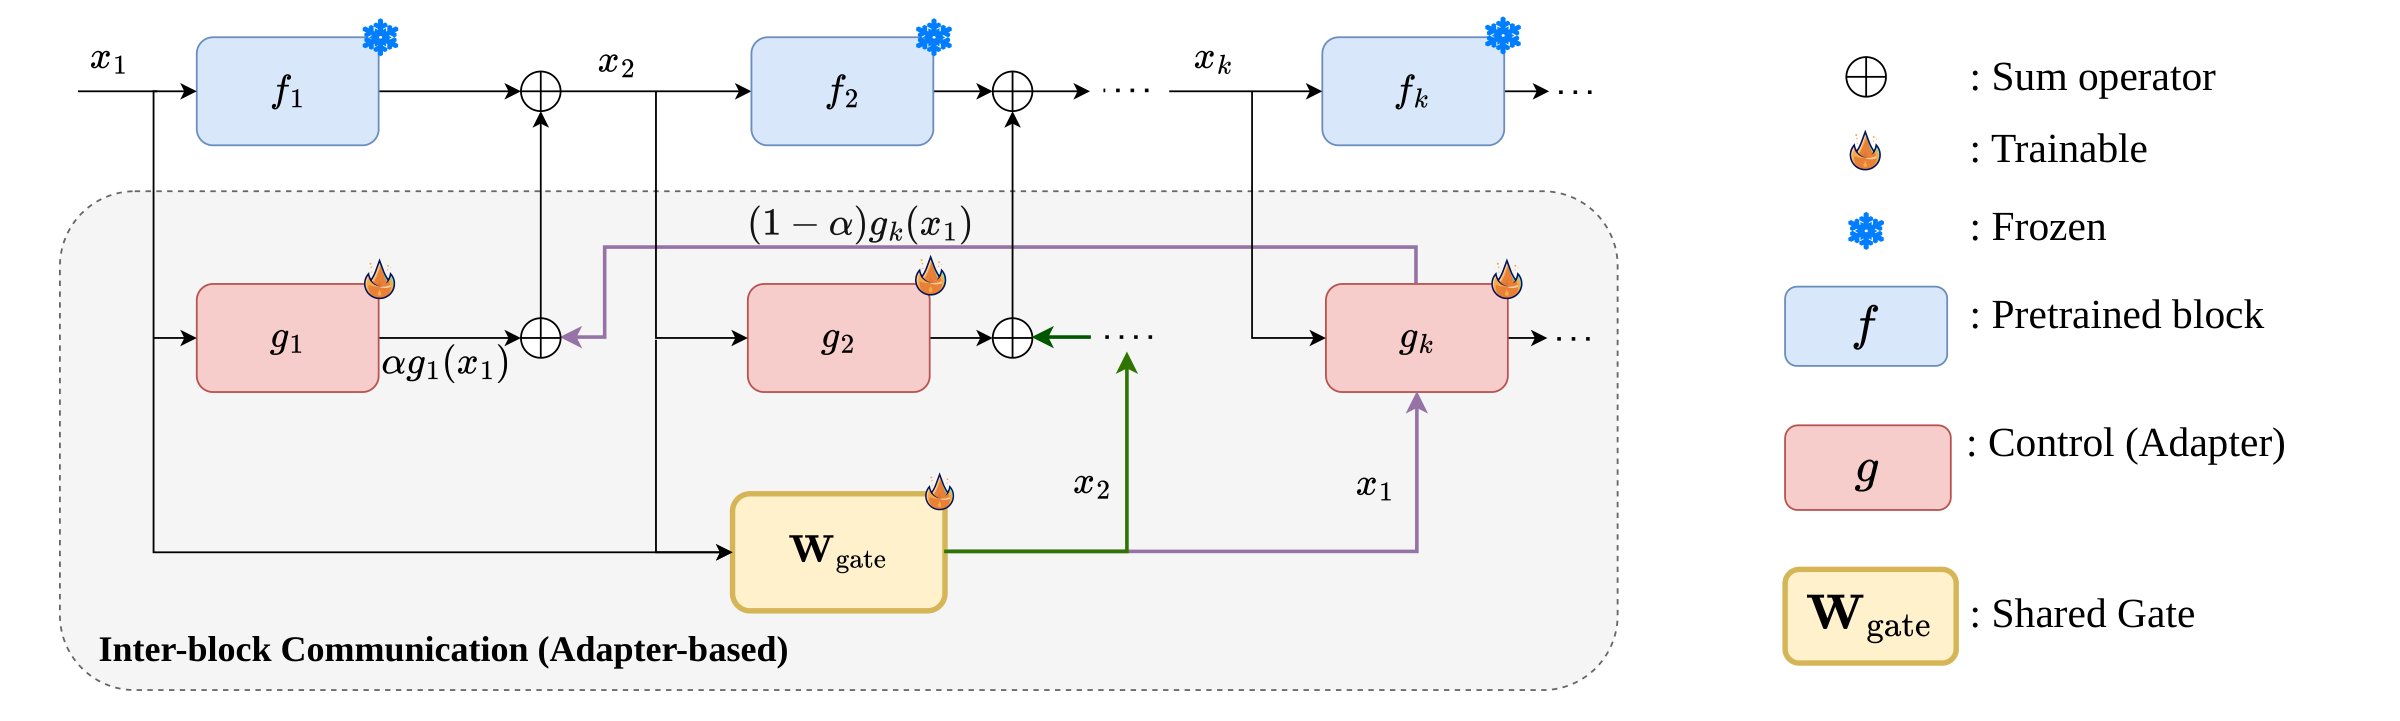
\includegraphics[width=0.96\linewidth]{MoC-project-page/static/images/MoC_architecture.png}
      \caption{At block $t$, the shared gate selects Top-$K$ controls from all
      layers and fuses the routed signal with the local controller. Frozen
      pretrained blocks are never re-run.}
    \end{figure}

    \heading{Sparse, shared routing}
    \[
      \pi_k(x_t)=\operatorname{softmax}
      \!\left(\operatorname{TopK}(\mathbf W_{\rm gate}x_t)\right)_k,
    \]
    \[
      x_{t+1}=x_t+f_t(W_tx_t)+\alpha g_t(x_t)
      +(1-\alpha)\sum_{k=1}^{L}\pi_k(x_t)g_k(x_t).
    \]

    All $L$ controls form one expert pool. One gate is shared across layers;
    load balancing prevents collapse. Training uses batch-level routing, while
    inference routes each sample from its own prefix.

    \heading{Forward pass at block $t$}
    Compute $p_{\rm own}=g_t(x_t)$; select and renormalize the Top-$K$ gate
    scores; aggregate $p_{\rm route}=\sum_{i\in S_K}\pi_i g_i(x_t)$; then fuse
    $g_{\rm MoC}=\alpha p_{\rm own}+(1-\alpha)p_{\rm route}$.

  \end{block}

  \begin{block}{5. What makes MoC work?}
    \begin{figure}
      \centering
      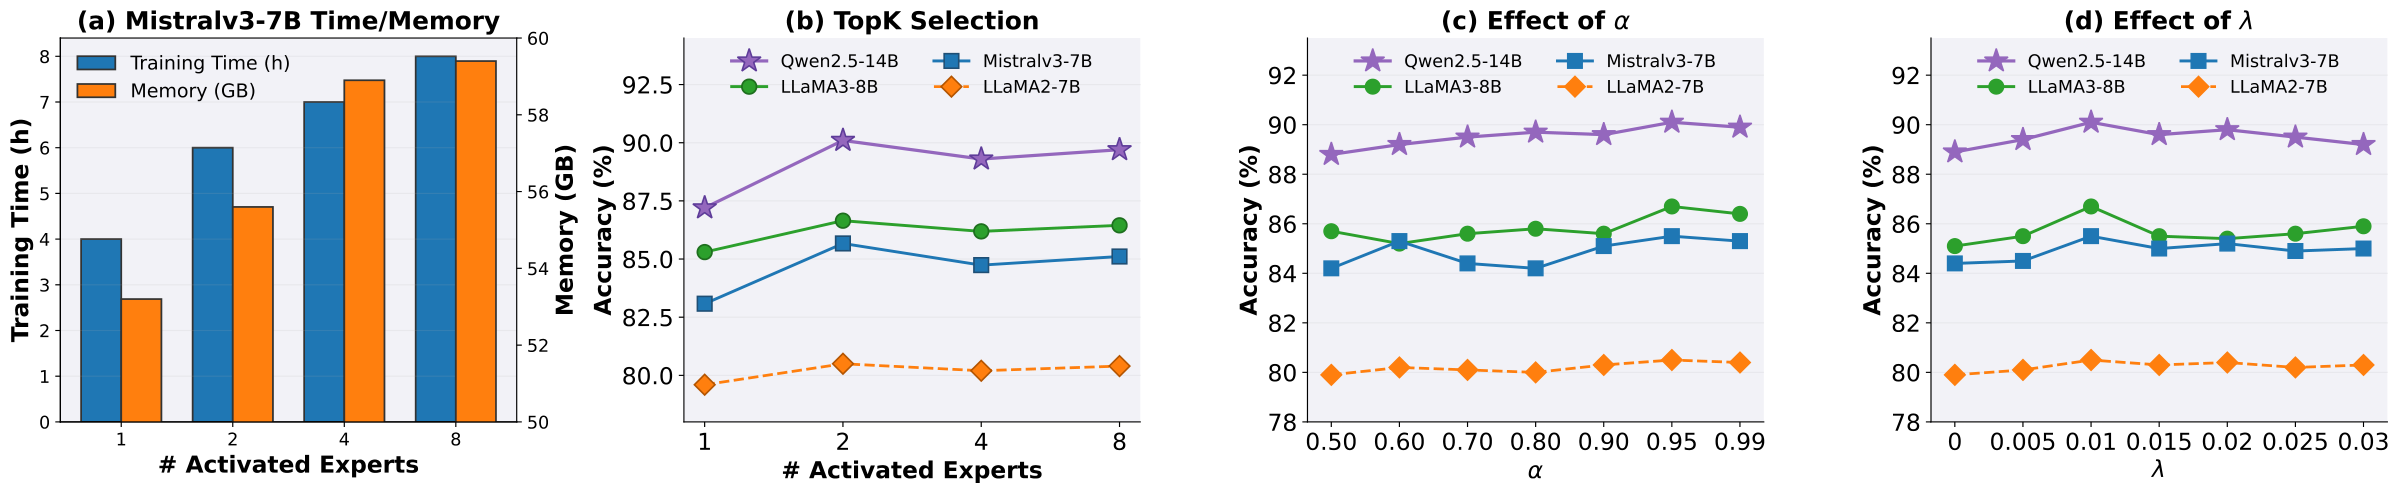
\includegraphics[width=0.97\linewidth]{MoC-project-page/static/images/ablation_hyperparams.png}
      \caption{Two activated experts work best (the local controller plus one
      routed expert). MoC is robust to $\alpha$ and peaks at $\alpha=0.95$;
      load balancing peaks at $\lambda=0.01$.}
    \end{figure}

    \begin{tabularx}{\linewidth}{X c c}
      \toprule
      \textbf{Cross-layer design} & \textbf{Avg. acc.} & \textbf{Memory} \\
      \midrule
      Local Control & 83.1 & 53.2 GB \\
      Uniform Control & 84.3 & 53.8 GB \\
      Fixed Control & 84.2 & 55.0 GB \\
      MoC without load balancing & 84.4 & 55.4 GB \\
      \textbf{MoC} & \textbf{85.5} & 55.6 GB \\
      \bottomrule
    \end{tabularx}

    \vspace{0.8ex}
    Adaptive routing improves by \textbf{+2.4 points} over local Control, with
    only 2.4 GB additional training memory. A shared ATTN+FFN gate is the best
    variant (86.7 on LLaMA3-8B; 85.5 on Mistralv3-7B).

  \end{block}

  \begin{alertblock}{Default configuration}
    \centering
    \textbf{Top-$K=1$ routed expert} $+$ local control \quad\textbullet\quad
    $\alpha=0.95$ \quad\textbullet\quad $\lambda_{\rm balance}=0.01$ \\
    Shared gate across attention and FFN control pathways.
  \end{alertblock}

\end{column}

\separatorcolumn

% ====================
% Column 3: results and takeaways
% ====================

\begin{column}{\colwidth}

  \begin{block}{6. Main results}

    \heading{Average accuracy on 8 commonsense datasets}
    \begin{table}
      \centering
      \begin{tabularx}{\linewidth}{X c c c c}
        \toprule
        \textbf{Method} & \textbf{LLaMA2} & \textbf{LLaMA3} & \textbf{Mistral} & \textbf{Qwen2.5} \\
        \midrule
        LoRA & 77.6 & 80.8 & 80.2 & 87.7 \\
        MoLEx & 78.9 & 81.5 & 81.3 & 87.8 \\
        Parallel Control & 79.6 & 85.3 & 83.1 & 87.2 \\
        \textbf{MoC} & \textbf{80.5} & \textbf{86.7} & \textbf{85.5} & \textbf{90.1} \\
        \bottomrule
      \end{tabularx}
      \caption{MoC achieves the best average on every LLM backbone. It also
      obtains the best averages on GLUE and VTAB-1K.}
    \end{table}

    \heading{Qwen2.5-14B: accuracy versus training cost}
    \begin{table}
      \centering
      \begin{tabularx}{\linewidth}{X c c c c}
        \toprule
        \textbf{Method} & \textbf{Params} & \textbf{Acc.} & \textbf{Time} & \textbf{Memory} \\
        \midrule
        LoRA & 0.63\% & 87.7 & 9.4 h & 62.1 GB \\
        MoLEx & 0.64\% & 87.8 & 20.3 h & 124.8 GB \\
        Parallel Control & 0.43\% & 87.2 & 6.5 h & 58.7 GB \\
        \textbf{MoC} & \textbf{0.43\%} & \textbf{90.1} & \textbf{8.0 h} & \textbf{61.3 GB} \\
        \bottomrule
      \end{tabularx}
    \end{table}

    \begin{center}
      \metric{+2.3}{accuracy points}{over MoLEx}
      \hfill
      \metric{$-51\%$}{GPU memory}{versus MoLEx}
      \hfill
      \metric{$2.5\times$}{faster training}{versus MoLEx}
    \end{center}

  \end{block}

  \begin{block}{7. Efficient inference}
    \begin{figure}
      \centering
      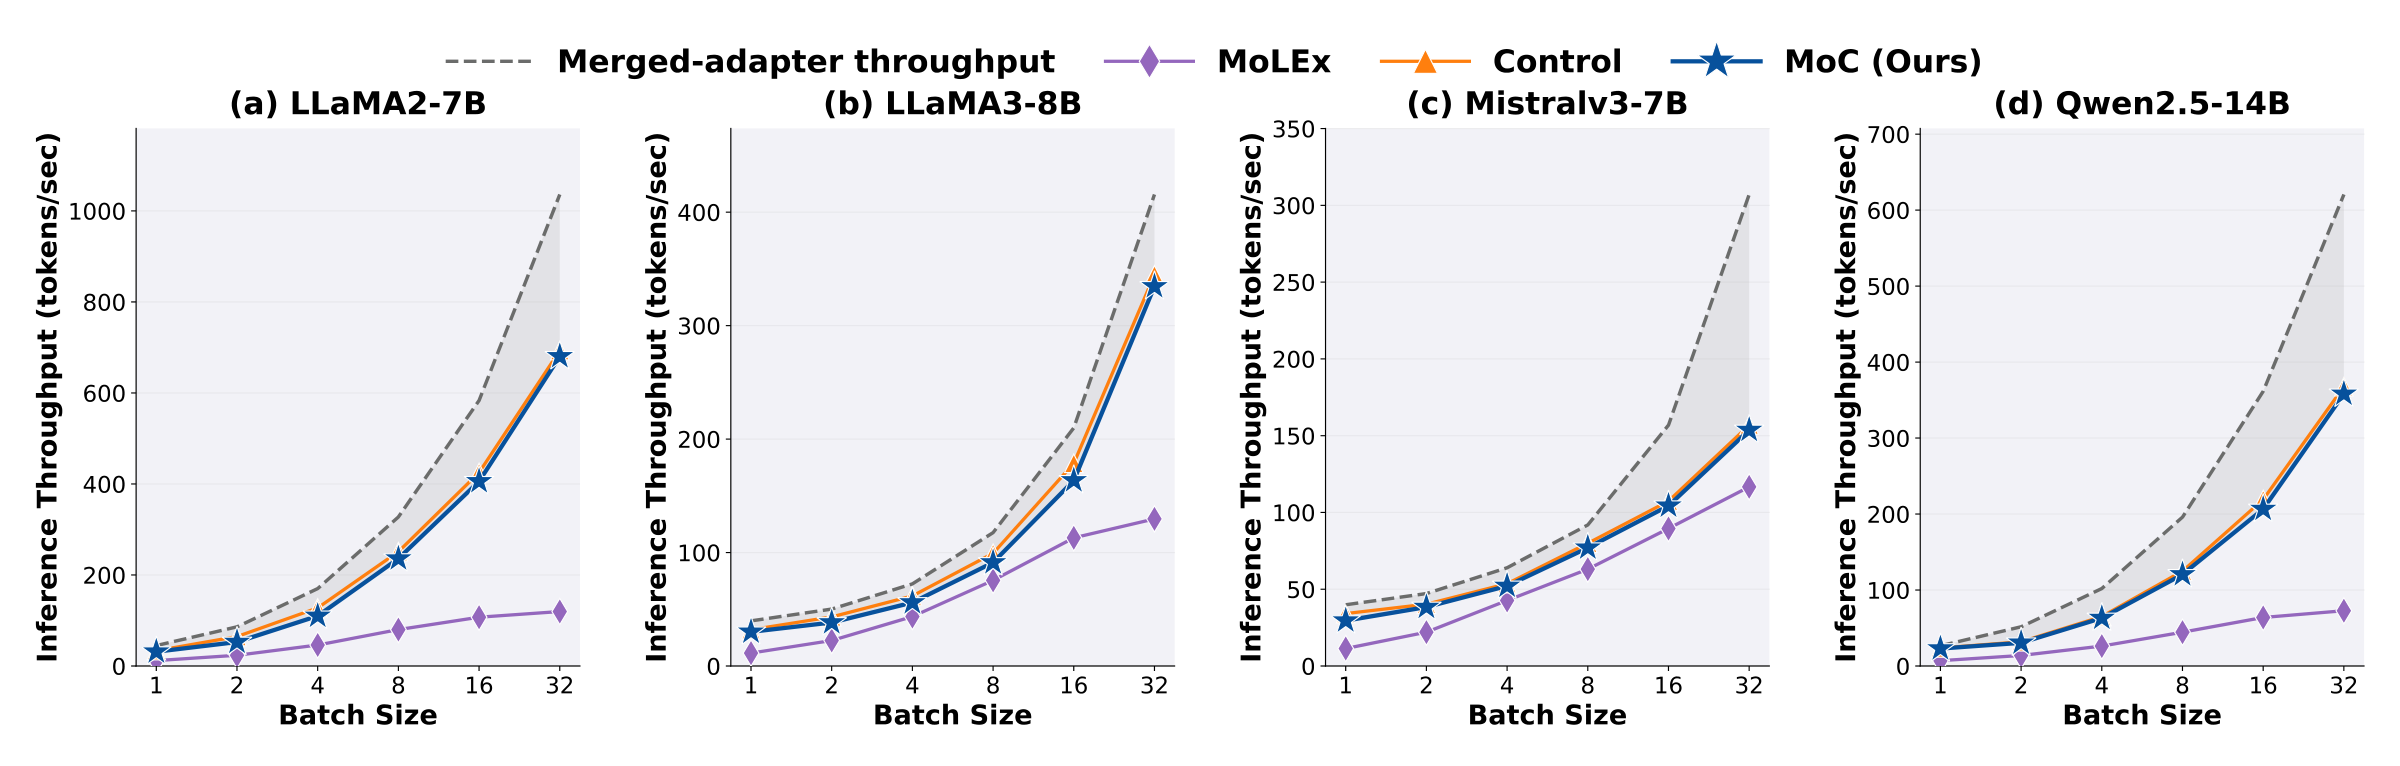
\includegraphics[width=\linewidth]{MoC-project-page/static/images/inference_throughput_moc_comparison.png}
      \caption{Across four LLMs and batch sizes, MoC stays close to Parallel
      Control and far above MoLEx. Mergeable weight adapters provide the shaded
      upper bound.}
    \end{figure}
  \end{block}

  \begin{block}{Takeaways and resources}
    \begin{columns}[c,totalwidth=\linewidth]
      \begin{column}{0.73\linewidth}
        \begin{itemize}
          \item \textbf{Mechanism:} sparse routing turns block-wise controls into
            a cross-layer expert pool.
          \item \textbf{Efficiency:} communication happens through lightweight
            states; pretrained blocks run only once.
          \item \textbf{Evidence:} MoC consistently improves state-based tuning
            across language and vision backbones.
          \item \textbf{Routing:} selected experts often come from distant layers,
            with task-dependent patterns.
        \end{itemize}

        \footnotesize
        \textbf{Paper:} \href{\arxivurl}{arXiv:2606.31397} \quad
        \textbf{NeurIPS:} \href{\paperurl}{poster \#148178}

        \vspace{0.5ex}
        Conducted in part at Qualcomm AI Research, an initiative of Qualcomm
        Technologies, Inc.
      \end{column}
      \begin{column}{0.23\linewidth}
        \centering
        \qrcode[height=5.4cm]{\arxivurl}\\[0.5ex]
        \footnotesize\bfseries Scan for paper
      \end{column}
    \end{columns}
  \end{block}

\end{column}

\separatorcolumn
\end{columns}
\end{frame}

\end{document}
